\chapter{Especificación de Requisitos}
\label{enlaceespecificacion}

Para proceder a especificar los requisitos se ha realizado un profundo análisis de los objetivos de la aplicación. Estos requisitos se han buscado teniendo en cuenta aspectos funcionales, de rendimiento, de seguridad, de información, etc.
\\

Las plantillas empleadas para las tablas de los requisitos y casos de uso se encuentran en los apéndices: la \hyperref[enlaceFRQX]{D.1. Plantilla de requisitos funcionales}, la \hyperref[enlaceNFRX]{D.2. Plantilla de requisitos no funcionales}, la \hyperref[enlaceIRQX]{D.3. Plantilla de requisitos de información} y la \hyperref[enlaceUCX]{D.4. Plantilla de Casos de uso}.
Estas plantillas están inspiradas en las tablas empleadas en el REM \cite{rem} para la Gestión de requisitos.
\\

La importancia de los requisitos será medida según el grado de la necesidad del requisito en la aplicación, siendo en el caso de este proyecto "Vital" para los requisitos de mayor importancia, yo "Quedaría bien" para los menos importantes. Por su parte, la urgencia, indicará aquellas partes que se han de implementar con mayor rapidez, siendo "Inmediatamente" aquellas que tienen una mayor prioridad, y "Puede esperar" los requisitos que no son extrictamente necesarios.

\section{Requisitos funcionales}

Los requisitos funcionales \cite{requisitos} son aquellos que definen una funcionalidad del sistema de software o sus componentes, tanto para las entradas de datos como para el comportamiento en situaciones específicas.
\\

En el caso de esta aplicación se han localizado dos grupos de requisitos funcionales: los asociados con operaciones de usuarios, y los que se relacionan con operaciones asociadas a leyes.
\\

Los requisitos funcionales pueden ser consultados en el \hyperref[APRequisitosFuncionales]{Apéndice C.1. Requisitos funcionales}.
\section{Requisitos no funcionales}
\label{APRequisitosNoFuncionales}

\begin{table}[H]
\begin{center}
\begin{tabular}{|p{3cm}|p{10cm}|} \hline
\centering {\bf NFR-01} & Tiempo de respuesta $<$ 2 segundos  \\ \hline\hline
\centering {\bf Versión} & 1.0 (05/06/2022) \\ \hline
\centering {\bf Descripción} & El sistema deberá responder en menos de 2 segundos, sin tener en cuenta el tiempo que tarde la red en enviar la información de vuelta al usuario. \\ \hline
\centering {\bf Importancia} & Vital \\ \hline
\centering {\bf Urgencia} & Inmediatamente \\ \hline
\end{tabular}
\caption{Requisito no funcional 01. Tiempo de respuesta $<$ 2 segundos.}
\label{enlaceNFR1}
\end{center}
\end{table}

\begin{table}[H]
\begin{center}
\begin{tabular}{|p{3cm}|p{10cm}|} \hline
\centering {\bf NFR-02} & Los datos sensibles del usuario se almacenan encriptados  \\ \hline\hline
\centering {\bf Versión} & 1.0 (05/06/2022) \\ \hline
\centering {\bf Descripción} & El sistema deberá encriptar los datos sensibles del usuario como las contraseñas en la base de datos de lex.gal. Se utilizará un algoritmo SHA-256 para encriptar. \\ \hline
\centering {\bf Importancia} & Vital \\ \hline
\centering {\bf Urgencia} & Inmediatamente \\ \hline
\end{tabular}
\caption{Requisito no funcional 02. Los datos sensibles del usuario se almacenan encriptados.}
\label{enlaceNFR2}
\end{center}
\end{table}

\begin{table}[H]
\begin{center}
\begin{tabular}{|p{3cm}|p{10cm}|} \hline
\centering {\bf NFR-03} & No permitir que un rol realice operaciones de otro  \\ \hline\hline
\centering {\bf Versión} & 1.0 (05/06/2022) \\ \hline
\centering {\bf Descripción} & El sistema deberá restringir aquellas operaciones exclusivas del administrador para el resto de usuarios. \\ \hline
\centering {\bf Importancia} & Vital \\ \hline
\centering {\bf Urgencia} & Inmediatamente \\ \hline
\end{tabular}
\caption{Requisito no funcional 03. No permitir que un rol realice operaciones de otro.}
\label{enlaceNFR3}
\end{center}
\end{table}

\begin{table}[H]
\begin{center}
\begin{tabular}{|p{3cm}|p{10cm}|} \hline
\centering {\bf NFR-04} & Permanecer operativo durante el horario de trabajo \\ \hline\hline
\centering {\bf Versión} & 1.0 (05/06/2022) \\ \hline
\centering {\bf Descripción} & El sistema deberá permanecer operativo durante todo el horario de trabajo de los empleados de lex.gal.  \\ \hline
\centering {\bf Importancia} & Vital \\ \hline
\centering {\bf Urgencia} & Inmediatamente \\ \hline
\end{tabular}
\caption{Requisito no funcional 04. Permanecer operativo durante el horario de trabajo.}
\label{enlaceNFR4}
\end{center}
\end{table}

\begin{table}[H]
\begin{center}
\begin{tabular}{|p{3cm}|p{10cm}|} \hline
\centering {\bf NFR-05} & Tratamiento de documentos en lenguajes de etiquetas  \\ \hline\hline
\centering {\bf Versión} & 1.0 (05/06/2022) \\ \hline
\centering {\bf Descripción} & El sistema deberá restringir el tratamiento de documentos a documentos escritos en lenguajes de etiquetas, como HTML o XML. \\ \hline
\centering {\bf Importancia} & Vital \\ \hline
\centering {\bf Urgencia} & Inmediatamente \\ \hline
\end{tabular}
\caption{Requisito no funcional 05. Tratamiento de documentos en lenguajes de etiquetas.}
\label{enlaceNFR5}
\end{center}
\end{table}

\begin{table}[H]
\begin{center}
\begin{tabular}{|p{3cm}|p{10cm}|} \hline
\centering {\bf NFR-06} & Tiempo de aprendizaje por el usuario $<$ 1h  \\ \hline\hline
\centering {\bf Versión} & 1.0 (05/06/2022) \\ \hline
\centering {\bf Descripción} & El sistema deberá tener un proceso de aprendizaje rápido y sencillo para el usuario, que en todo caso deberá ser menor de 1 hora. \\ \hline
\centering {\bf Importancia} & Vital \\ \hline
\centering {\bf Urgencia} & Inmediatamente \\ \hline
\end{tabular}
\caption{Requisito no funcional 06. Tiempo de aprendizaje por el usuario $<$ 1h.}
\label{enlaceNFR6}
\end{center}
\end{table}

\begin{table}[H]
\begin{center}
\begin{tabular}{|p{3cm}|p{10cm}|} \hline
\centering {\bf NFR-07} & Proporcionar mensajes de apoyo al usuario  \\ \hline\hline
\centering {\bf Versión} & 1.0 (05/06/2022) \\ \hline
\centering {\bf Descripción} & El sistema deberá proporcionar mensajes de apoyo al usuario en todas las operaciones, con el objetivo de facilitar la navegación en la aplicación. \\ \hline
\centering {\bf Importancia} & Quedaría bien \\ \hline
\centering {\bf Urgencia} & Puede esperar \\ \hline
\end{tabular}
\caption{Requisito no funcional 07. Proporcionar mensajes de apoyo al usuario.}
\label{enlaceNFR7}
\end{center}
\end{table}

\begin{table}[H]
\begin{center}
\begin{tabular}{|p{3cm}|p{10cm}|} \hline
\centering {\bf NFR-08} & Uso de tecnologías web y servicios RESTful  \\ \hline\hline
\centering {\bf Versión} & 1.0 (05/06/2022) \\ \hline
\centering {\bf Descripción} & El sistema deberá emplear tecnologías web para realizar la aplicación, incluyendo HTML5, Tailwind como framework de CSS y React.js como framework de JavaScript. Además, todos los servicios serán RESTful, y serán implementados con Spring Boot. \\ \hline
\centering {\bf Importancia} & Vital \\ \hline
\centering {\bf Urgencia} & Inmediatamente \\ \hline
\end{tabular}
\caption{Requisito no funcional 08. Uso de tecnologías web y servicios RESTful.}
\label{enlaceNFR8}
\end{center}
\end{table}

\begin{table}[H]
\begin{center}
\begin{tabular}{|p{3cm}|p{10cm}|} \hline
\centering {\bf NFR-09} & Base de datos NoSQL  \\ \hline\hline
\centering {\bf Versión} & 1.0 (05/06/2022) \\ \hline
\centering {\bf Descripción} & El sistema deberá almacenar todos los datos en una base de datos NoSQL de MongoDB. \\ \hline
\centering {\bf Importancia} & Vital \\ \hline
\centering {\bf Urgencia} & Inmediatamente \\ \hline
\end{tabular}
\caption{Requisito no funcional 09. Base de datos NoSQL.}
\label{enlaceNFR9}
\end{center}
\end{table}

\begin{table}[H]
\begin{center}
\begin{tabular}{|p{3cm}|p{10cm}|} \hline
\centering {\bf NFR-10} & Generación de tokens JWT  \\ \hline\hline
\centering {\bf Versión} & 1.0 (05/06/2022) \\ \hline
\centering {\bf Descripción} & El sistema deberá generar tokens JWT cada vez que un usuario inicie sesión en la aplicación. De esta forma, los datos del usuario no quedan tan accesibles en la web, y será necesario utilizar un algoritmo  {\it hash} para desencriptarlos. En todo caso la contraseña no será almacenada en el token JWT. \\ \hline
\centering {\bf Importancia} & Vital \\ \hline
\centering {\bf Urgencia} & Inmediatamente \\ \hline
\end{tabular}
\caption{Requisito no funcional 10. Generación de tokens JWT.}
\label{enlaceNFR10}
\end{center}
\end{table}
\section{Requisitos de información}

Por último, los requisitos de información \cite{requisitos}, son aquellos requisitos que indican algún tipo de información, la cual es necesaria para el correcto funcionamiento del sistema.
\\

En el caso de esta aplicación, se han localizado dos: Usuario y Documento.
\\

Los requisitos de información pueden ser consultados en el \hyperref[APRequisitosInformacion]{Apéndice C.3. Requisitos de información}.
\section{Casos de uso}

Un caso de uso \cite{casodeuso} es cualquier acción o actividad que se realiza en el sistema. Representan diferentes operaciones que se realizan en la aplicación.
\\

Los casos de uso pueden ser consultados en el \hyperref[APCasosUso]{Apéndice C.4. Casos de uso}.
\section{Interfaz con la API del DOG}

En el caso de este TFG, las leyes son importadas de la API del DOG. Para ello se accede a través de un servicio web el cual ha sido implementado con el objetivo de acceder a esta API, y así poder obtener los datos de las leyes necesarios.
\\

Estas leyes pueden ser filtradas por parte del usuario de la aplicación, para proceder posteriormente a importarla a la base de datos de lex.gal, y así poder trabajar con ellas.

\begin{figure}[H]
\centerline{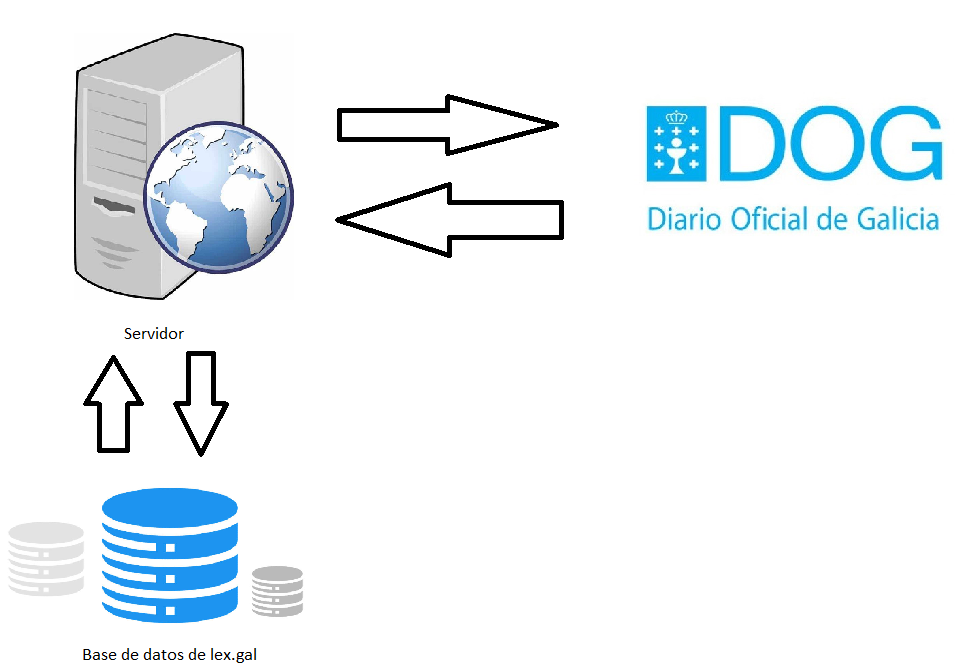
\includegraphics[width=10cm]{figuras/interfazDOG.png}}
\caption{Interfaz entre el servidor, la base de datos de lex.gal y la API del DOG.}
\label{enlaceInterfazDOG}
\end{figure}